\chapter{Background}


\section{Natural language Processing}
Language requires a whole batch of preprocessing steps to account for the redundancy in language and facilitate the otherwise not accessible underlying rules (including but not limited to grammar). For this purpose, a pipeline has been established.

\textcolor{red}{Here comes a image of a NLP pipeline}


\subsection{Corpus}

\subsection{Stop Words}
Assuming we want to analyze text on the level of words, we might be looking for
words that appear more often than others. This information can tell us a lot about the topic or sentiment of the text. Suppose we find that a text is frequently mentioning \textit{brexit} more than any other word. Then we can deduct, that this text might be a (news) article and that it is talking about one of the most controversial disputes of the European Union as of March 2019. However, we quickly realize that certain words also appear more frequently than others, without revealing much about the content of the text. Words like \textit{the, of, than} appear numerously in every English text independently of the topic or the source. Stop words already received particular attention in \citeyear{Luhn1960} where their property to obscure target words that are actually important for further analyzes was identified. These words are called \textbf{stop words}\index{stop words}.

In case we want to find, as an example, any adverb in a text, then we would not want to discard words that help localizing adverbs.Every word in this context has some information about the grammatical structure of the text and thus must be taken into consideration. But, if we should be interested in the topic or source of the text, then we might end up searching for this semantic information within only a handful of words. In this case, it would only distract our learner, classification algorithm, or other machine learning tool if the vast majority of words would not transmit the information of interest. Therefore, it is common practice to remove stop words for classification algorithms \citep{McCallum1998, Lodhi2002, Tong2001} but not for state-of-the-art neural classifier as in \citep{Howard2018}.

\subsection{Regular Expressions}
Regular expressions (\gls{regex}) is a syntax using ASCII characters to describe a set of strings matching this syntax. Regex consist of meta and literal characters. For a literal character holds that it elicits the search for this exact character within a regex when the regex is interpreted. A meta-character is interpreted and has a special role in defining regexs \citep{Kleene1951}. While these metacharacter vary between different regex libraries, certain ones are preserved along all of them. A literal character combined with a \texttt{*} is a very common functionality (known as the Kleene star) with different regexs and means that the literal character may appear $0$ to $n$ time to allow a match. To still be able to use those metacharacter as literal characters, they can be escaped with a backslash. Many of the following concepts are based on rules formulated as regexs.

\subsection{Tokenization}
A token is an abstraction of a piece of information consisting of a byte representation for some symbol. In NLP this can be a single character, word, punctuation, or sentences. The goal in \textbf{tokenization}\index{tokenization} is
to split text into meaningful chunks that obey the rules of the language which defines what a single word or sentence or character mean. Word-tokenization is the cornerstone for the vast majority of NLP analyzes.
Nevertheless, token are rather loosely connected to what we perceive as an atomic unit in language and we need to keep in mind that in the case of computers it is just an representation of some (hopefully) UTF-8 code.

Token not always match how we think about words. It could be that the word \textit{U.S.A.} is split into six tokens \{\textit{U}, \textbf{.}\,, \textit{S}\,, \textbf{.}\,, \textit{A}\,, \textbf{.}\} or \textit{don't} into \{\textit{do}, \textit{n't}\} although we know it should be \{\textit{do}, \textit{not}\} when tokens are a representation of words. But since tokens are not meant to be representation of words but rather a method to yield word level understanding then \textit{not} represented as \textit{n't} will not worsen any text analysis, if the usage of \textit{n't} is consistent. However, splitting the acronym \textit{U.S.A.} into six token discards a large amount of information and cannot be allowed. A solution is typically usgin a combination of a curated list of expected abbreviations and special to avoid confusing them for the ending of a sentence. Alternatively, one could train a unsupervised sentence boundary detector as described in \cite{Kiss2006}. By binning occurrences of ending a sentence, this method extracts the most occurring sentence breaks, and learns to discard those, that do not to seem be a valid new sentence. The acronym \textit{U.S.A.} will occur only as a fraction compared to more frequent sentence breaks in which lower-case letters are followed by a whitespace, a period, and then a upper-case letter. An very simple regex for sentence-tokenization would be \texttt{[a-z] \textbackslash.[A-Z]}.

A simple regex for word tokenization would be \texttt{[a-z,A-Z]+} that matches 1 to $n$ (indicated by \texttt{+}) character to the set (indicated by \texttt{[ ]}) of lower or uppercase letter.

Sentence tokenization is based on word-tokenization and is also part of most text analyzes. It becomes important for example if a text includes logical parts (like paragraphs or chapters) that need to be handled differently.
These two methods facilitate almost all important methods in NLP \citep{Webster1992}.

\subsection{POS-Tagging}
Although task like text classification perform already well with an text that only has been tokenized, mostly we require further processing of our raw text. If the grammatical correction of text is the goal of our NLP pipeline then it goes without saying that we need more information about the grammatical functionality of our extracted token. Assume an sentence like \textit{``I read a book about grammar that were very helpful"}. An lookup of all token/words would yield that every word is written correctly but the sentence is still wrong. We know that \textit{that} refers to \textit{book} and that \textit{book} is singular and a singular relative pronoun must not be followed by a plural auxiliary verb (in this case \textit{are}). A simple lookup is not able to detect \textit{that} should be followed by \textit{is} since \textit{that} is written the same when referring to plural nouns. To solve this programmatically, we could implement a lookup of the grammatical number of the noun before the first mentioning of \textit{that} to determine if the grammatical count of the auxiliary verb after \textit{that} is correct. To find the noun, we apply \textbf{position-of-speech tagging}\gls{POS-tagging}. A POS-tagger is typically a machine learning model like a decision tree \citep{Marquez98} trained on annotated corpus like \citep{PennTreebank}, that already has the right grammatical entities assigned to each word in unstructured texts.

\subsection{Lemmatization and Stemming}
Assuming we have found a method to apply tokenization with a satisfying performance then we might want to start some simple descriptive statistics about the text. We could count the amount of word-tokens in the text, or determine the longest token found. The simplest way to sensibly reason about a text would be to find the most occurring words. They most likely will be \textit{the}, \textit{a} or punctuations but we already know about stop words so we remove them. Without them, the word count could help us infer the subject of a text. If our goal was to infer the type of sport based on the most occurring words in sports news and we might find a high occurrence of players' names. If we are not able to link players' names to a sport we then hope to find a large term frequency for something like \textit{throw} for baseball or \textit{strike} for soccer. This, unfortunately, will not be the case when only counting tokens in a text. The words in the text will occur in many forms due to grammatical conjugation. For example \textit{thrown} and \textit{throw} will be treated as unequal token for the computer although they mean the same. What we need is, to transform all words to their infinitive form.

There are to options: \textbf{stemming}\index{stemming} and \textbf{lemmatization}\index{lemmatization}. Stemming only prunes the end of words following rules. These rules are specified as regular expression and try to exploit regularities in language to infer the infinitive form. However, they will not always reliably work due to special cases and ambiguities. One common rule among stemmers is the removal of \textit{ing} at the end of a word to transform a word to its infinitive form. This works in many cases but fails for words like \textit{lying} that is transformed to \textit{ly} which is programmatically wrong.

Lemmatization uses more sophisticated approaches. First, it uses a look-up instead of rules and therefore will be able to correctly transform \textit{lying} to \textit{lie}. Second, it in-cooperates POS-tagging to determine whether the word to lemmatize is a verb or a noun \citep{Muller2015}. If i.e. \textit{meeting} is a noun, than we do not want to transform it to \textit{meet} but keep it like it is. Nowadays, where computational speed is often not of utmost concern, lemmatization is preferred over stemming since it is more accurate\citep{Balakrishnan2014}.


\subsection{Bag Of Words}\label{section:bow}
In a machine learning task it is preferable to use the large size of data as a leverage to avoid doing explicit feature engineering. Instead of having any domain knowledge, it is preferred to let the algorithm pick the features. One apparent example for this in NLP is the \textbf{bag of words}\index{bag of words} approach. It is very difficult to model language because of its entangled grammar, all its special cases, idioms, and ambiguity (i.e. \textit{bank}). Therefore, we try to analyze a text based only on the occurrences of the words in the text. The grammatical context for these words is omitted which means that we only focus on the words used. We do so by tokenizing our text, lemmatize the token and operate on the set of words left after this preprocessing. A common example for the performance of this simple model is spam detection. Given a set of emails and labels \emph{spam} and \emph{not spam}, a machine learning model could learn these labels based on the presence of words based on the learned word distributions of the labels.

\subsection{(Disease) Name Entity Recognition}
Name entity recognition (\GLS{NER}) is a step placed towards the end of a NLP pipeline. After sentences and words have been tokenized, and POS-tagging was applied, it might be important for certain learning algorithms to
know the entity of the word at hand. Common examples are the recognition of names for persons or companies and for numerical entities, like time, dates and money \citep{Nadeau2009}. This recognition might be part of some NLP pipeline but it also can be part of a pipeline for information retrieval (\GLS{IR}). The work steps of IR is the extraction of specific information and their subsequent storage in a database with the objective to structure large amount of data that is difficult to access \citep{Manning2008, Wei2011}.

The reason NER is not simply covered by a lookup but a separate module in a pipeline, is the difficulty to deal with ambiguous words as \textit{apple}. When the word \textit{Apple} is at the beginning of a text, it is unclear whether it stands for the fruit or a billion dollar company. While in the beginning NER consisted of handcrafted rules and heuristics \citep{Rau1991}, NER is now a classification problem that is solved through supervised learning, capable of learning relationships with Hidden Markov Models, Decision Trees, or Conditional Random Fields \citep{Nadeau2009} Though, there is a shift towards non/semi-supervised methods that infer features (as neural networks) and outperform feature-engineered systems (as decision trees) \citep{Yadav2018}.

In the medical field such ambiguities rise not because the proper names are so indistinguishable from other common words, but because there are many forms how to write a disease name and equally many abbreviations (i.e. \textit{cancer}, \textit{carcinoma}, \textit{malignant tumor}, \textit{CA}). To reason from medical text, it is important to identify those utterances that are most likely representing a disease. Thus, disease-NER is a important processing step in this domain. However, benchmarks also showed that in highly standardized text lookups perform equally well \citep{Jimeno2007}. Therefore, the exact procedure to perform DNER depends on the sources that need to be processed.

\section{Machine Learning}
Machine learning (\GLS{ML}) is the attempt to make computer learn. \citeauthor{Mitchell1997} described learning broadly as,
%
\begin{quote}
``A computer program is said to \textbf{learn} from experience $\mathcal{E}$ with respect to some class of task $\mathcal{T}$ and performance measure $\mathcal{P}$, if its performance at tasks in $\mathcal{T}$, as measured by $\mathcal{P}$, improves with experience $\mathcal{E}$''
\end{quote}
%
There are, however, ML algorithms that not necessarily have $\mathcal{E}$ defined (unsupervised methods). Therefore, one could also consider the following definition  \[f: X \rightarrow y\] where $f$ is our machine learning model that takes our data $X$ and tries to predict the most likely label $\hat{y}$ where $\hat{y} \approx y$ and $y$ being the true label.

\subsection{Naive Bayes Classifier}\label{section:nbc}
The \textbf{naive Bayes classifier}\index{naive Bayes classifier} (\GLS{NBC}) is a probabilistic classifier. It describes a set of algorithms capable to learn inferring a label given a set of features. These algorithms are trained in a supervised fashion. The NBC is defined as :

\begin{align}
  \boldsymbol{x} &= \{x_1, x_2, \dots, x_n\} \\
  \mathcal{C} &= \{\mathcal{C}_k \: | \: k \in K \} \\
  P(\mathcal{C}_k|\boldsymbol{x}) &= \frac{P(\boldsymbol{x} |\mathcal{C}_k) P(\mathcal{C}_k)} {P(\boldsymbol{x})} \\
  P(\mathcal{C}_k|\boldsymbol{x}) &\propto \frac{P(x_1 |\mathcal{C}_k)
                                       P(x_2 |\mathcal{C}_k) \dots
                                       P(x_n |\mathcal{C}_k)
                                       P(\mathcal{C}_k)}{ P(\boldsymbol{x})}
\end{align}

Where $\boldsymbol{x}$ is our data point which consists of $n$ features. Note, the the classifier is named \textsl{naive} because we assume that every feature in our vector $\boldsymbol{x}$ is independent, i.e. there is no correlation between them. This most of the time is wrong but in practice the NBC still performs very well \citep{Rish2001}. $\mathcal{C}$ is the set of all our classes. The goal of the NBC is to predict the probability of our data point $\boldsymbol{x}$ belonging to a class $\mathcal{C}_k$. Hence, to predict the class $\boldsymbol{x}$ belongs to. A common procedure is to find the maximum a posteriori (MAP) probability
\begin{gather}
  \argmax_{k \in \mathcal{C}} P(\mathcal{C}_k|\boldsymbol{x})
\end{gather}
to build a classifier.
 Solving $P(\boldsymbol{x} |\mathcal{C}_k)$ in (2.3) is hard and requires a huge amount of data form all classes to predict the most likely set of features denoted as $\boldsymbol{x}$ reliably. But since we assumed independence of our features, we can rewrite (2.4) due to the chain rule as
 \[p(x_i| \{\forall x_j \in \boldsymbol{x} : j \neq i \}, \mathcal{C}_k) \overset{x_i\perp\!\!\!\perp \forall x_j}{\Longleftrightarrow} p(x_i|\mathcal{C}_k)\]
 To evaluate (2.4), we simply need to take the product of the probabilities of the features given the label and then evaluate the classification as in (2.5).

\subsubsection{Multinomial Naive Bayes}
%TODO: Add tf-idf
In the case for having a discrete features, like in a document, we can apply multinomial naive Bayes like:
\begin{align}
  \mathcal{C} &= \{\mathcal{C}_k \: | \: k \in K \} \\
  \boldsymbol{t} &= \{c_1, c_2, \dots, c_n\} \\
  \boldsymbol{T} &= \{\boldsymbol{t}_d | \forall d \in \mathcal{D}\} \\
  p({t_{i}}|\mathcal{C}_k) &= \frac{\boldsymbol{T}_{\mathcal{C}_k,t_{i}}}{\sum_{\forall t_j \in \boldsymbol{T}}\boldsymbol{T}_{\mathcal{C}_k,t_j}} \\
  P(\mathcal{C}_k|\boldsymbol{t}_d) &\propto P(\mathcal{C}_k) \prod_{i=1}^{|t_{d}|}  p(t_{d,i}|\mathcal{C}_k)
\end{align}
Where $\mathcal{C}$ is again our set of classes, and $\boldsymbol{t}$ the set of token counts where $c_n$ is the occurrence count of term $n$. $\boldsymbol{T}$ is a matrix where the token counts $c$ are the columns, and the documents $d$ the rows. To calculate the likelihood $P({t_{i}}|\mathcal{C}_k)$ we simply divide the occurrence of token $t_i$ given class $\mathcal{C_k}$ by the sum of all tokens in the same class. Following the independence assumption as in (2.4) we now can calculate $P(\mathcal{C}_k\boldsymbol{t}_d)$ as the product of the prior $P(\mathcal{C}_k)$ - the probability of class $\mathcal{C}_k$
as learned form the training set - and the probabilities of all the terms $t_{1 \dots n}$ given the prior class. For classification, the $\argmax$ as in (2.5) is taken.

Two problems can occur in text classification that need to be handled. First, the high probability of numerical underflow due to the large product of several values $<1$, and second, we need to account for some token $t_i \in \boldsymbol{t_d}$ having a count of $0$ that would nullify the whole product. The solution to the underflow problem is to transform (2.10) in to log-space which equals to:
%
\[log(P(\mathcal{C}_k|\boldsymbol{t}_d)) \propto \log(P(\mathcal{C}_k)) + \sum_{i=1}^{|t_{d}|} \log({p(t_{d,i}|\mathcal{C}_k)}) \]
%
To avoid $p({t_{i}}|\mathcal{C}_k)$ becoming $0$ we apply Laplace smoothing\index{Laplace smoothing} to (2.9) which yields
\[p({t_{i}}|\mathcal{C}_k) = \frac{\boldsymbol{T}_{\mathcal{C}_k,t_{i}} + 1}{\sum_{\forall t_j \in \boldsymbol{T}}(\boldsymbol{T}_{\mathcal{C}_k,t_j} + 1)}\]
\subsubsection{Bernoulli Naive Bayes}
Especially for shorter texts, there is no gain to count tokens, but rather treat them as binary values (present, not present). This explicitly model the absence and presence of words where we can model the probability of token $t_i$ given a some class like
\[p(t_{i}|\mathcal{C}_k) = p(t_{i})(1-p(t_{i}))^{(1-b_{i})}\]

\subsubsection{Complement Naive Bayes}
There are cases where the \textsl{naive} assumption is ill made. In a unbalanced class problem, the data is skewed towards the larger class which the following table illustrates,

\begin{table}[h!]
  \centering
  \caption{An coin flip example with a imbalanced class. $\theta$ is the probability of a class to yield head ($H$). Per experiment we flip one coin in $Class 1$ and two coins ins $Class 2.$ Then the label $H$ is assigned to one of both classes. Adopted from \cite{Rennie2003}}
  \setlength{\tabcolsep}{1.5em}
  \begin{tabular}{@{}cccc@{}}
    % $\theta_{Class 1} = 0.25$ &  $\theta_{Class 2} = 0.25$ & $p(data)$ & Label for H \\
    % \hline
    % T & TT & $0.48$ & $none$ \\
    % T & \{HT, TH\} & $0.24$ & $Class 2$ \\
    % T & HH & $0.03$ & $Class 2$ \\
    % H & TT & $0.16$ & $Class 1$ \\
    % H & \{HT, TH\} & $0.08$ & $Class 1$ \\
    % H & HH & $0.01$ & $none$
    \toprule
    \textbf{Class 1} & \textbf{Class 2} & $\mathbf{p(data)}$ & \textbf{Label for H} \\
    $\theta = 0.25$ & $\theta=0.2$ & & \\
    \midrule
    T & TT & $0.48$ & $none$ \\
    T & \{HT, TH\} & $0.24$ & $Class 2$ \\
    T & HH & $0.03$ & $Class 2$ \\
    H & TT & $0.16$ & $Class 1$ \\
    H & \{HT, TH\} & $0.08$ & $Class 1$ \\
    H & HH & $0.01$ & $none$ \\
    \bottomrule
  \end{tabular}
  \label{table:coinflip}
\end{table}
The experiment shown in table \ref{table:coinflip} , that considers each possible outcome of coin flips, suggests a 24\% probability for $Class 1$ to yield $H$ and 27\% for $Class 2$, although the probability for $Class 1$ to yield $H$ is actually higher.
The proposed solution by \cite{Rennie2003} is to minimize the probability of a vector of word counts not belonging to a class,
\[\argmin P(\neg\, \mathcal{C}_k) \prod_{i=1}^{|t_{d}|} \frac{1}{p(t_{d,i}|\neg\, \mathcal{C}_k)} \]

\subsection{Deep Learning}
\subsubsection{Perceptron}
A \textbf{perceptron}\index{perceptron} is an algorithm inspired by biological neurons. It is a binary classifier that is learns by adjusting its threshold to \textsl{fire} an \textsl{action potential} when the correct class is detected. Formally it is
\begin{gather}
  Perceptron(\mathbf{x}) = \begin{cases}1 & \text{if }\ \mathbf{w} \cdot \mathbf{x} + \mathbf{b} > 0,\\
  0 & \text{otherwise}\end{cases}
\end{gather}
where $\mathbf{x}$ is our data vector, $w$ the weight vector and $b$ the bias where $w$, $b$, and $x$ are of same length. It is trained in a supervised fashion. The learning step with which $w$ is adjusted is defined as,
\[\mathbf{w}(t+1) = \mathbf{w}(t) + \eta (\mathbf{d}(t) - \mathbf{y}(t))\mathbf{x}(t)\]
with $\mathbf{d}$ being the training data vector and $\mathbf{y}$ the corresponding label vector at training step $t$ with a learning rate $\eta \in (0,1]$.
\subsubsection{Multi Layer Perceptron}
A \textbf{multi layer perceptron} (\GLS{MLP}\index{multi layer perceptron}) (Fig. )\ref{fig:MLP}) consists of three layers, an input and output layer, and $1 \dots n$ hidden layers. Each layer consists of a perceptron. The activation function is not a Boolean function but as sigmoid function $\sigma(y) = \frac{1}{1+e^{-y}}$. Its output also ranges from $0$ to $1$ but is derivable. Derivablity is crucial since the MLP uses backpropagation to be trained. Described by,
\begin{align}
  E(\mathbf{w})_t &\equiv \frac{1}{2} \sum (\mathbf{d}_t - \mathbf{y}_t)^2 \\
  \Delta \mathbf{w} &= - \eta \frac{\delta E_t}{\delta \mathbf{w}}
\end{align}
where $E$ is the sum over of the errors over all output neurons at step $t$ and $\Delta \mathbf{w}$ is the weight adjustment according to the backproagated error $\frac{\delta E_t}{\delta \mathbf{w}}$ that is the partial derivative of the error given all the weights with a learning rate $\eta$. The minus sign indicates that the weight is adjusted downwards the estimated gradient (minimization).


\begin{figure}[h!]
  \centering
  \begin{tikzpicture}[shorten >=1pt,->,draw=black!50, node distance=\layersep]
      \tikzstyle{every pin edge}=[<-,shorten <=1pt]
      \tikzstyle{neuron}=[circle,fill=black!25,minimum size=17pt,inner sep=0pt]
      \tikzstyle{input neuron}=[neuron, fill=green!50];
      \tikzstyle{output neuron}=[neuron, fill=red!50];
      \tikzstyle{hidden neuron}=[neuron, fill=blue!50];
      \tikzstyle{annot} = [text width=4em, text centered]

      % Draw the input layer nodes
      \foreach \name / \y in {1,...,4}
      % This is the same as writing \foreach \name / \y in {1/1,2/2,3/3,4/4}
          \node[input neuron, pin=left:Input \y] (I-\name) at (0,-\y) {};

      % Draw the hidden layer nodes
      \foreach \name / \y in {1,...,5}
          \path[yshift=0.5cm]
              node[hidden neuron] (H-\name) at (\layersep,-\y cm) {};

      % Draw the output layer node
      \node[output neuron,pin={[pin edge={->}]right:Output}, right of=H-3] (O) {};

      % Connect every node in the input layer with every node in the
      % hidden layer.
      \foreach \source in {1,...,4}
          \foreach \dest in {1,...,5}
              \path (I-\source) edge (H-\dest);

      % Connect every node in the hidden layer with the output layer
      \foreach \source in {1,...,5}
          \path (H-\source) edge (O);

      % Annotate the layers
      \node[annot,above of=H-1, node distance=1cm] (hl) {Hidden layer};
      \node[annot,left of=hl] {Input layer};
      \node[annot,right of=hl] {Output layer};
  \end{tikzpicture}
  \caption{A illustration of a multi layer perceptron. The input (green), hidden (purple), and output (red) layer are each perceptrons. The arrow indicate the direction of the computation of the input which is a scalar.}
  \label{fig:MLP}
\end{figure}
\subsubsection{Convolutional Neural Network}
While the MLP is only capable to receive a single vector as an input, the \textbf{convolutional neural network}(\GLS{CNN})\index{convolutional neural network} is able to process a matrix. The additional dimension can then represent time or spatial dependencies. The extracted features are not represented by single neurons throughout hidden layers, but are adopted to so called feature maps. Feature maps are small (smaller than the input) matrices where their entries are weights that are adjusted during the training process. These feature maps are striding over the input and apply a convolution,
\[C(i,j) = (I \ast F)(i,j) = \sum_m \sum_n I(m, n) F(i-m, j-n)\] where $\ast$ is the convolutional operator, $I$ is our input matrix, $F$ the feature map, and $C(i,j)$ the output for the convolution at position $(i,j)$ of our feature map. The output matrix $C$ of the convolution step is then pooled which is i.e., the max or average value of $C$. This process can be repeated when several pooling steps commit to a new matrix. At the end, a fully connected layer (a MLP where every neuron is connected with each neuron) incorporates all information and yields a classification (Fig. \ref{fig:cnn}).
\begin{figure}[h!]
    \centering
    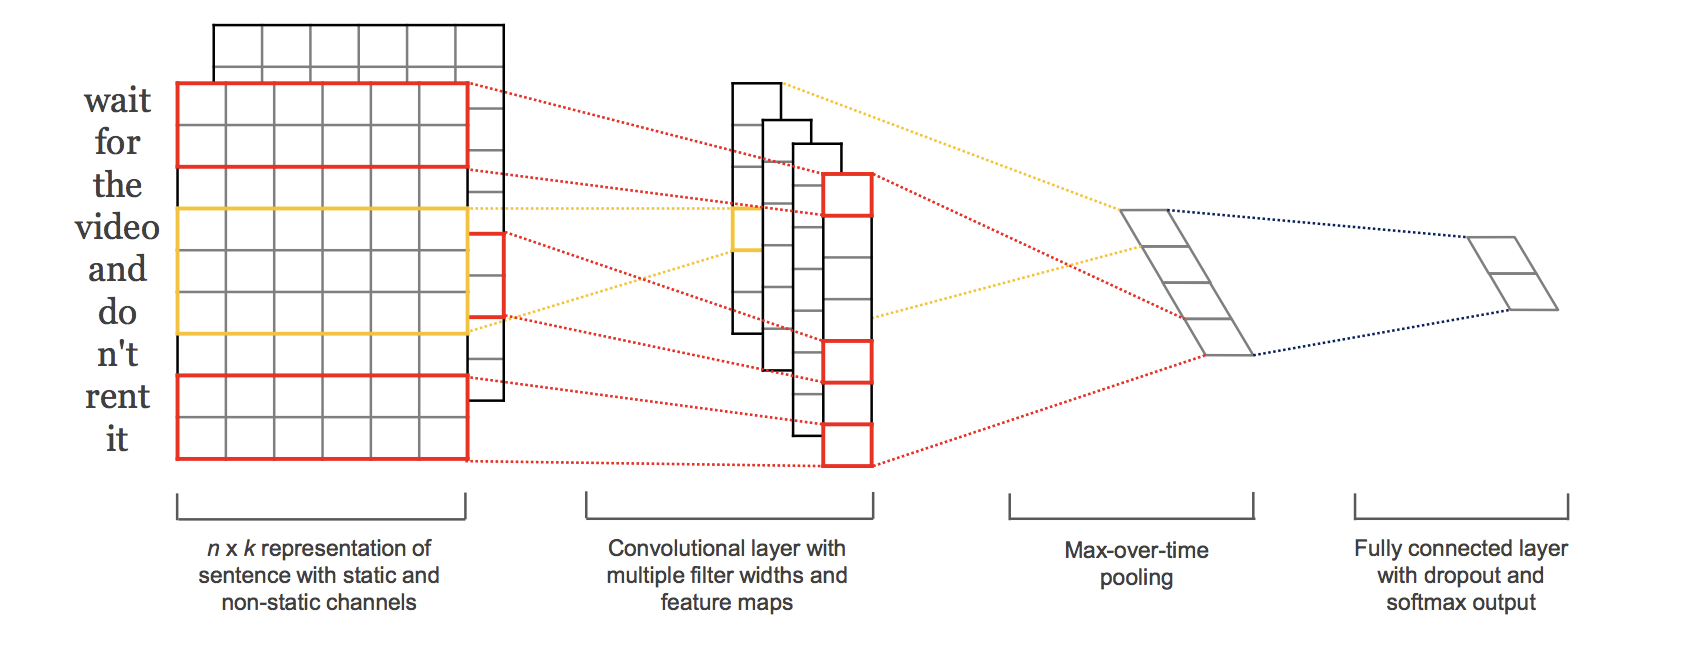
\includegraphics[scale=0.5]{CNN.png}
    \caption{An illustration of a n-gram convolutional neural network. The input is a numerical representation (\ref{section:embeddings}) of a tokenized text. The convolution over the input matrix is represented as a red and yellow box (called feature map) that is then pooled (i.e. max of the kernel). The classification is then enforced by a fully connected layer that incorporates the input of all feature maps.}
    \label{fig:cnn}
\end{figure}


\subsection{Embeddings}\label{section:embeddings}
In \ref{section:bow} I have been pointing out that using the bag-of-words approach is explained by the difficulty to explicitly model language and in \ref{section:nbc} I showed that this approach does not hurt the performance of the classifier. However, bag of words models language incorrectly and having a better representation of language improves our ML algorithms. Word embeddings are a method to represent words as n-dimensional vectors to much better capture syntactic and semantic characteristics of language.
\subsubsection{Word2Vec}
In 2013 two algorithms to efficiently compute high quality distributed representations of words and phrases were published. A synonym for this approach is \textbf{word2vec}\index{word2vec}. The general approach is both algorithms to maximize the similarity measures of words that appear in a similar context. The \textbf{continues bag-of-words model}\index{continues bag-of-words model} is trained to predict the vector representation of a word or phrase given  $n$ words before and after the word in a sentence. A slower implementation with the benefit to model infrequent words better is the \textbf{continuous skip-gram-model}\index{continuous skip-gram-model} \citep{word2vec}. The skip-gram-model tries to predict the context given a word and is thus the opposite approach of the bag-of-words model. In practice we generate labeled data of the form of tuples, where one entry is the target word $\mathbf{w}_t$ and the other entries are context words $\mathbf{w}_c$ such that the tuple is $(\mathbf{w}_t, \mathbf{w}_{c_{1}}, \dots, \mathbf{w}_{c_{n}})$. The tuple can either contain actual context words found in the text, or random words from the vocabulary (negative sampling). The embedding layer learns the weights of the input and context words, by yielding a n-dimensional vector for all of these words, calculate a dot-product of both vectors in the merge-layer and then pass it to a sigmoid layer that predicts whether the words are actual context words or have been negatively sampled. In short, the objective of the algorithm is to maximize
\[\sum_{t \in T} \sum_{c \in \mathcal{C}_t} log( p(\mathbf{W}_c|\mathbf{w}_t))\]
where $\mathbf{w}$ is the vector representation of a word. $t$ is the target word and $\mathbf{W}_c$ the context matrix, where each row is a vector representation of a context word.
\subsubsection{GloVe}
\subsubsection{BERT}
\subsubsection{Document Embedding}

\subsection{Web Scraping}
\subsubsection{DOM}
\subsubsection{Ajax}
\subsubsection{REST}
